\documentclass[11pt,a4paper]{article}
\usepackage{acl2015}
\usepackage{times}
\usepackage{url}
\usepackage{latexsym}
\usepackage{enumerate}
\usepackage[utf8]{inputenc}
\usepackage[spanish]{babel} 
\usepackage{graphicx}
\usepackage{multirow}
\usepackage{float}
\restylefloat{table}

\title{Categorizaci\'on de Tweets en Español por Variedad y Genero. Asignatura Text Mining en Social Media. Master Big Data}

\author{Alejandro Uzc\'ategui Cort\'es \\
  {\tt alejandrouzc@gmail.com} \\}

\date{}

\setlength{\parskip}{2mm}

\begin{document}
\maketitle
\begin{abstract}
El presente artículo trata el estudio del author profiling, aplicándolo a un caso práctico de clasificación tweets en español por género y variedad del español del autor. Para el análisis y estudio del caso se decidió hacer una exploración de los datos para encontrar las palabras más frecuentes y partiendo de estas observaciones se crearon y usaron distintos vocabularios en la generación de bolsas de palabras, técnica elegida para aplicar los modelos de aprendizaje y realizar las predicciones. Se obtuvieron buenos resultados usando las técnicas de Support Vector Machines, árboles C5.0 y Random Forest. A partir del trabajo realizado y los resultados se plantearon posibles pruebas a futuro para mejorar aún más la técnica.

\textit{Palabras clave: author profiling, vocabularios, bolsas de palabras, modelos de aprendizaje.}
\end{abstract}


\section{Introducción}
  El author profiling se basa en analizar una cantidad de textos o documentos para descubrir características del autor, de acuerdo al estilo en el que escribe y el contenido de los textos. Esta técnica ha ganado gran importancia y sigue aún creciendo con aplicaciones importantes en áreas como mercadeo y análisis forense y de seguridad.

En este trabajo, se procesarán textos obtenidos de Twitter para aplicar author profiling. Los tweets a analizar están escritos en español, pero con distintas variaciones del idioma debido que los autores de los tweets recopilados provienen de los siguientes países: Argentina, Chile, Colombia, España, México, Perú y Venezuela. También es de importancia tener en cuenta que, además de la variación de nacionalidad, los autores son de distinto género. El problema planteado consiste en clasificar los tweets recopilados por variedad de español de acuerdo al país de procedencia del autor y por genero del mismo, utilizando técnicas y modelos de predicción para así poder realizar el author profiling.

\section{Dataset}

El caso de estudio propuesto cuenta con un dataset compuesto de tweets en español de autores de distinto género y nacionalidad. A continuación, se presentan algunas características básicas del dataset: 

\begin{itemize}
\item Tamaño del dataset: 279999 tweets.
\item Tweets por género:
  \begin{itemize}
	\item Femenino: 139999
	\item Masculino: 140000
  \end{itemize}
\item Tweets por país:
  \begin{itemize}
	\item Argentina: 40000
	\item Chile: 40000
	\item Colombia:  40000
	\item España: 39999
	\item México: 40000
	\item Perú: 40000
	\item Venezuela: 40000
  \end{itemize}
\item Autores por género: 
  \begin{itemize}
	\item Femenino: 1400
	\item Masculino: 1400
  \end{itemize}
\item Autores por país:
  \begin{itemize}
	\item Argentina: 400
	\item Chile: 400
	\item Colombia:  400
	\item España: 400
	\item México: 400
	\item Perú: 400
	\item Venezuela: 400
  \end{itemize}
\end{itemize}

Para iniciar el análisis del caso, se realizó un pre-proceso del dataset y se generó un vocabulario con las palabras más frecuentes. Esto consiste en leer los tweets y aplicar una serie de transformaciones para tratar de normalizarlos lo más posible; dichas transformaciones incluyen: pasar todo el tweet a minúsculas, remover signos de puntuación, remover números, quitar espacios en blanco y quitar palabras de parada comunes del idioma. Al final se obtiene un vocabulario con los términos más usados y su frecuencia. 

A partir de lo observado aquí, se planteó la idea de crear vocabularios separados tanto por género como por variedad para ver como se comportaba cada grupo y si proporcionaba información de interés para el análisis. Se generaron wordclouds que permitieran tener una mejor visualización de los términos y así poder comparar fácilmente entre las clases estudiadas. A continuación, se presenta como ejemplo el wordcloud obtenido para tweets de autores del género femenino:

\begin{figure}[h!]
  \centering
    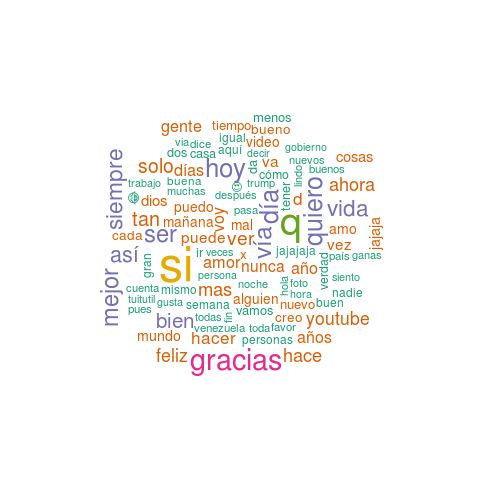
\includegraphics[width=0.4\textwidth]{0Female}
  \caption{Wordcloud de palabras más frecuentes del género femenino}
\end{figure}

Tanto en este como en el resto de los wordclouds de las otras clases se observo que habían palabras que se repetían en todos, por lo que se decidió graficar las frecuencias de las veinte palabras mas usadas para ver que tanto peso tenían estas en cada caso. Por ejemplo, para tweets de autores del género femenino:

\begin{figure}[h!]
  \centering
    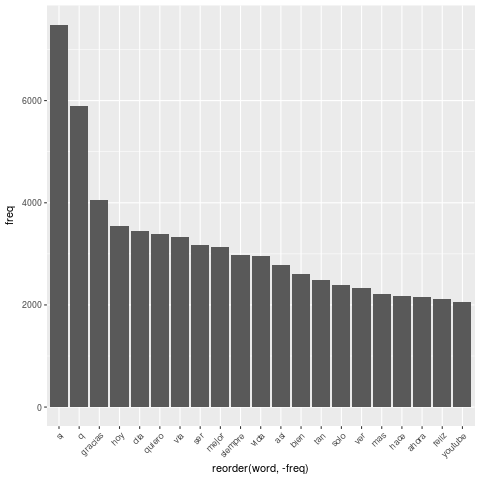
\includegraphics[width=0.4\textwidth]{00Female-barras}
  \caption{Gráfica con frecuencia por palabra de las veinte palabras más frecuentes del género femenino}
\end{figure}

Se evidenció que existían palabras con frecuencias demasiado elevadas, en comparación con el resto, repetidas en todas las clases por lo que se decidió generar una lista de palabras a ser excluidas de los vocabularios a usar para la predicción; puesto que sin estas se tendría una mejor muestra a la hora de probar los modelos de aprendizaje. La lista esta comprendida por las palabras: si, q, d, x, hoy, gracias, vía, ser.

\section{Propuesta del alumno}

Para el entrenamiento de modelos y predicción de los resultados se decidió trabajar con distintas combinaciones de vocabularios para generar bolsas de palabras o bag of words (en adelante referidas como BoW), puesto es la técnica con la que más familiarización se contaba y con que se pudo obtener resultados válidos.

Primero, se generó un vocabulario genérico, sin eliminar las palabras de la lista creada en la exploración del dataset. Se crearon BoWs, por género y variedad, con las que se hicieron pruebas iniciales de los modelos; pudiendo así observar cuales aportaban los mejores resultados. Los modelos usados fueron: support vector machines (svm), naive bayes (nb), árboles c5.0 (c50), vecinos cercanos (knn) y random forest (rf). En esta prueba se obtuvieron resultados pésimos para nb y knn por lo que se decidió obviarlos y proceder con el resto.

En cuanto a la identificación de variedad del español sólo se trabajó con BoWs partiendo del vocabulario con la lista de palabras especiales removidas y utilizando los modelos previamente mencionados. Se obtuvieron resultados bastante buenos que serán presentados en el próximo apartado.

En el caso de la identificación de género también se usaron BoWs pero con dos tipos de vocabularios diferentes. El primero, es el mismo usado para las pruebas de variedad. Para la segunda prueba, se decidió crear un vocabulario especial que contuviese solamente las palabras más frecuentes usadas por las mujeres que a su vez no fuesen usadas por los hombres y viceversa. 

Cabe destacar que se realizaron pruebas con otras técnicas y características, como por ejemplo n-gramas y longitud de los tweets, pero que no se pudieron aplicar bien por lo que no se obtuvieron resultados de las mismas.

\section{Resultados experimentales}

Para el caso de la variedad se obtuvieron los siguientes resultados:

\begin{table}[H]
\centering
\begin{tabular}{|c|l|l|}
\hline
n                     & \multicolumn{1}{c|}{Model} & \multicolumn{1}{c|}{Accuracy} \\ \hline
\multirow{3}{*}{1000} & SVM                        & 0.7721                        \\ \cline{2-3} 
                      & C5.0                       & 0.7621                        \\ \cline{2-3} 
                      & RF                         & 0.8936                              \\ \hline
\multirow{3}{*}{500}  & SVM                        & 0.705                         \\ \cline{2-3} 
                      & C5.0                       & 0.75                          \\ \cline{2-3} 
                      & RF                         & 0.8579                        \\ \hline

\end{tabular}
\caption{Resultados de la predicción de la variedad del español del autor}
\end{table}

Se hicieron dos rondas de prueba variando el n con los distintos modelos. Es evidente que, con muy poca manipulación de los datos se obtienen buenos resultados. Con random forest y un n de 500 se logro superar el baseline indicado.

Los resultados para la identificación de género son los siguientes:

\begin{table}[H]
\centering
\begin{tabular}{|c|c|l|l|}
\hline
Vocabulary               & n                     & \multicolumn{1}{c|}{Model} & \multicolumn{1}{c|}{Accuracy} \\ \hline
\multirow{2}{*}{general} & \multirow{3}{*}{1000} & SVM                        & 0.6586                        \\ \cline{3-4} 
                         &                       & C5.0                       & 0.6764                        \\ \hline
\multirow{7}{*}{género}  & \multirow{3}{*}{185}  & SVM                        & 0.7064                        \\ \cline{3-4} 
                         &                       & C5.0                       & 0.6657                        \\ \cline{3-4} 
                         &                       & RF                         & 0.6964                        \\ \cline{2-4} 
                         & 285                   & RF                         & 0.6986                        \\ \cline{2-4} 
                         & 395                   & SVM                        & 0.6886                        \\ \cline{2-4} 
                         & \multirow{2}{*}{595}  & SVM                        & 0.685                         \\ \cline{3-4} 
                         &                       & C5.0                       & 0.6757                        \\ \hline
\end{tabular}
\caption{Resultados de la predicción del género del autor}
\end{table}

Se puede notar que el género es un problema más difícil que la variedad del idioma, lo que se refleja claramente en los resultados. Con las pruebas realizadas con el vocabulario general se obtuvieron valores muy próximos al baseline, tanto por encima como por debajo del mismo; y con el vocabulario de género si se logró en todas las variaciones de n superar el baseline propuesto.

Es evidente que, con muy poca manipulación de los datos y el uso de una técnica sencilla como es BoW, se pueden alcanzar resultados bastante aceptables. Esto indica que, si se procesaran un poco más los datos o se crearán otras combinaciones de vocabularios, existe la posibilidad de seguir la mejora de resultados.

\section{Conclusiones y trabajo futuro}

Por medio de este trabajo se pudo apreciar lo interesante e importante que puede ser el author profiling, y como podía aplicarse a distintas áreas y problemas de estudio. Se obtuvo conocimientos de nuevas técnicas para el análisis de datos, al mismo tiempo que se reforzaron conocimientos previamente obtenidos. Sería de gran interés continuar estudiando esta área para ver que otras aplicaciones se le puede dar.

Como pruebas propuestas a futuro para continuar la mejoría de resultados, sería interesante intentar nuevamente el uso de n-gramas y la longitud de los tweets que no se pudieron implementar correctamente durante este trabajo. De igual forma, se proponen también otras posibilidades como estudiar el uso de hashtags, menciones y emojis; así como también otras características lingüísticas como el uso de preposiciones y adjetivos.


\end{document}
